Проблема  выбора структуры модели является фундаментальной в области машинного обучения и интеллектуального анализа данных.
Проблема выбора структуры модели глубокого обучения формулируется следующим образом: решается задача классификации или регрессии на заданной или пополняемой выборке $\mathfrak{D}$. Требуется выбрать структуру нейронной сети, доставляющей минимум ошибки на этой функции и максимум качества на некотором внешнем критерии.
 Под моделью глубокого обучения понимается суперпозиция дифференцируемых по параметрам нелинейный функций. Под структурой модели понимается значения структурных параметров модели, т.е. величин, задающих вид итоговой суперпозиции. 

Формализуем описанную выше задачу.
\begin{defin}
\textit{Объектом} назовем пару $(\x, y), \x \in \Xb =  \mathbb{R}^n, y \in \yb$. В случае задачи классификации $\yb$ является распределением вероятностей принадлежности объекта $\mathbf{x} \in \mathbb{X}$ множеству классов $\{1, \dots, R\}$: $\yb \subset [0,1]^R$, где $R$ --- число классов. В случае задачи регрессии $\yb$ является некоторым подмножеством вещественных чисел ${y} \in \yb  \subseteq \mathbb{R}$.
Объект состоит из двух частей: $\mathbf{x}$  соответствует \textit{признаковому описанию объекта}, $y$ --- \textit{метке объекта}.
\end{defin}

Задана простая выборка \begin{equation}\label{eq:dataset}\mathfrak{D} = \{(\mathbf{x}_i,y_i)\}, i = 1,\dots,m,\end{equation} состоящая из множества объектов $$\mathbf{x}_i \in \mathbf{X} \subset  \mathbb{X}, \quad {y}_i \in \mathbf{y} \subset \yb.$$ 


\begin{defin}
\textit{Моделью} $\mathbf{f}(\mathbf{w}, \mathbf{x})$ назовем дифференцируемую по параметрам $\mathbf{w}$ функцию из множества признаковых описаний объекта во множество меток:
\[
    \mathbf{f}:  \mathbb{W}  \times \mathbb{X} \to \yb,
\] 
где $\mathbb{W}$ --- пространство параметров функции $\mathbf{f}$.
\end{defin}
Специфика задачи  выбора модели \textit{глубокого обучения} заключается в том, что модели глубокого обучения могут иметь значительное число параметров, что приводит к неприменимости ряда методов оптимизации и выбора модели. 
Перейдем к формальному описанию параметрического семейства моделей глубокого обучения. 
\begin{defin}
Пусть задан ациклический граф $(V,E)$, такой что 
\begin{enumerate}
\item для каждого ребра $(j,k) \in E$: вектор базовых дифференцируемых функций  $\mathbf{g}^{j,k} = [\mathbf{g}^{j,k}_0, \dots, \mathbf{g}^{j,k}_{K^{j,k}-1}]$  мощности $K^{j,k}$;
\item для каждой вершины $v \in V$: дифференцируемая функция агрегации $\textbf{agg}_v$.
\item Функция $\mathbf{f} = \mathbf{f}_{|V|-1}$, задаваемая по правилу 
\begin{equation}
\label{eq:modelfam}
    \mathbf{f}_{k}(\mathbf{w}, \mathbf{x}) = \textbf{agg}_{k}\left(\{ \langle \boldsymbol{\gamma}^{j,k}, \mathbf{g}^{j,k} \rangle \circ  \mathbf{f}_j(\mathbf{x})| j \in \text{Adj}(v_k)\}\right), 
\end{equation}
\[
k \in \{1,\dots,|V|-1\}, \quad \mathbf{f}_0(\mathbf{x}) = \mathbf{x}, \quad v_k \in V. 
\]
и являющаяся функцией из признакового пространства $\mathbb{X}$ в пространство меток $\yb$ при значениях векторов, $\boldsymbol{\gamma}^{j,k} \in [0,1]^{K^{j,k}}$.
\end{enumerate}

Граф $(V, E)$ со множеством векторов базовых функций $\{\mathbf{g}^{j,k}, (j,k) \in E\}$ и функций агрегаций $\{\textbf{agg}_k\},$ где $k \in \{0, \dots, |V|-1\},$ назовем \textit{параметрическим семейством моделей} $\mathfrak{F}$.
\end{defin}

Примером функций агрегации выступают функции суммы и конкатенации векторов.

\begin{defin}
Функции $\mathbf{f}_0, \dots, \mathbf{f}_{|V|-1}$ из~\eqref{eq:modelfam} назовем \textit{слоями или подмоделями} модели $\mathbf{f}$.
\end{defin}

\begin{utv}
Для любого значения $\boldsymbol{\gamma}^{j,k} \in [0,1]^{K^{j,k}}$ функция $\mathbf{f} \in \mathfrak{F}$ является моделью.
\end{utv}
\begin{proof}
Утверждение следует непосредственно из определения: по условию утверждения для любого $\boldsymbol{\gamma}^{j,k} \in [0,1]^{K^{j,k}}$ функция является дифференцируемой функцией из признакового пространства $\mathbb{X}$ в пространство меток $\yb$, что соответствует определению модели.
\end{proof}



Пример параметрического семейства моделей, которое описывает сверточную нейронную сеть, представлена на Рис.~\ref{fig:scheme_cnn}. Семейство задает множество моделей с двумя операциями свертки с одинаковым размером фильтра $c_0$ и различным числом каналов $c_1$ и $c_2$. Единичная свертка с $c_1$ каналами $\textbf{Conv}(\mathbf{x}, c_1, 1)$ требуется для выравнивания размерностей скрытых слоев. Каждая модель параметрического семейства задается формулой: 
\[
    \mathbf{f} = \textbf{agg}_2\left(\left\{{\gamma}^{1,2}_0 \mathbf{g}^{1,2}_0 \left(\textbf{agg}_1 \left(\{{\gamma}^{0,1}_0 \mathbf{g}^{0,1}_0(\mathbf{x}), {\gamma}^{0,1}_1 \mathbf{g}^{0,1}_1(\mathbf{x})  \} \right)\right)\right\}\right).
\]
Положим, что функции агрегации $ \textbf{agg}_1,  \textbf{agg}_2$ являются операциями суммы. Заметим, что к вершине, соответствующей модели $\model_2$ ведет только одно ребро, поэтому операцию суммы можно опустить. 
Итоговая формула модели задается следующим образом:
\begin{multline*}
    \mathbf{f} = {\gamma}^{1,2}_0 \textbf{softmax} \bigl({\gamma}^{0,1}_0 \textbf{Conv}(\mathbf{x}, c_0, c_1)(\mathbf{x}) +\\ + {\gamma}^{0,1}_1 \textbf{Conv}(\mathbf{x}, 1, c_1) \circ \textbf{Conv}(\mathbf{x}, c_0, c_2)(\mathbf{x}) \w^{1,2}_0\bigr).
\end{multline*}



\begin{figure}
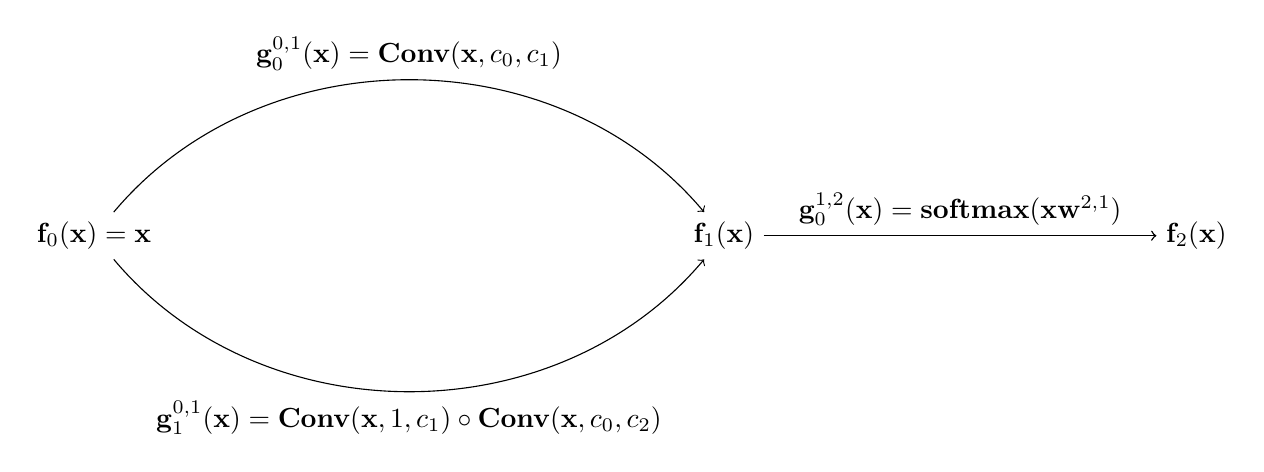
\begin{tikzpicture}[node distance=cm, auto]
  %\tikzstyle{every state}=[fill=red,draw=none,text=white]

  \node (f0)  at (1,6)                  {$\mathbf{f}_0(\mathbf{x}) = \mathbf{x}$};
  %\node (g11) at (6,3)                    {$\mathbf{g}^{1,1}(\mathbf{x})$};% = \text{Conv}(\mathbf{x}, 3, 32, 1)$};
  %\node (g12)  at (6,9)                   {$\mathbf{g}^{1,2}(\mathbf{x})$};% = \text{Conv}(\mathbf{x}, 4, 32, 1)$};
  \node (f1)  at (9,6)                 {$\mathbf{f}_1(\mathbf{x})$};% = \gamma^{1,1}\mathbf{g}^{1,1}(\mathbf{x}) +  \gamma^{1,2}\mathbf{g}^{1,2}(\mathbf{x})$};
  %\node (g21) at (12,6)                   {$\mathbf{g}^{2,1}(\mathbf{x})$};% = \boldsymbol{\sigma}(\mathbf{w}^{2,1}\mathbf{x})$};
  \node (f2)  at (15,6)                   {$\mathbf{f}_2(\mathbf{x})$};% = \gamma^{2,1}\mathbf{g}^{2,1}(\mathbf{x})$};
  \path[->]  (f0) edge [bend left=50] node {$\mathbf{g}^{0,1}_0(\mathbf{x}) = \textbf{Conv}(\mathbf{x}, c_0, c_1)$}(f1);
  \path[->] (f0)  edge[bend right=50] node[below] {$\mathbf{g}^{0,1}_1(\mathbf{x}) = \textbf{Conv}(\mathbf{x}, 1, c_1) \circ \textbf{Conv}(\mathbf{x}, c_0, c_2)$}(f1);
  \path[->] (f1)  edge node {$\mathbf{g}^{1,2}_0(\mathbf{x}) = \textbf{softmax}(\mathbf{x}\mathbf{w}^{2,1})$}(f2);            
  \draw[->] (f1) to (f2);
 
\end{tikzpicture}
\caption{Пример параметрического семейства моделей глубокого обучения: семейство описывает сверточную нейронную сеть.}
\label{fig:scheme_cnn}

\end{figure}




\begin{defin}
\textit{Параметрами }модели $\mathbf{f}$ из параметрического семейства моделей $\mathfrak{F}$  назовем конкатенацию векторов параметров всех базовых функций $\{\mathbf{g}^{j,k}| {(j,k) \in E} \}, \mathbf{w} \in \mathbb{W}.$ Вектор параметров базовой функции $\mathbf{g}^{j,k}_l$ будем обозначать как $\mathbf{w}^{j,k}_l$.
\end{defin}



\begin{defin}
Структурой $\boldsymbol{\Gamma}$  модели $\mathbf{f}$ из параметрического семейства моделей $\mathfrak{F}$  назовем конкатенацию векторов $\boldsymbol{\gamma}^{j,k}$. Множество всех возможных значений структуры $\boldsymbol{\Gamma}$ будем обозначать как $\amsmathbb{\Gamma}$.
Векторы $\boldsymbol{\gamma}^{j,k}, (j,k) \in E$ назовем \textit{структурными параметрами модели.}
\end{defin}

\begin{defin}
\textit{Параметризацией }множества моделей $M$ назовем параметрическое семейство моделей $\mathfrak{F}$, такое что для каждой модели $\mathbf{f} \in M$ существуют значение структуры модели $\boldsymbol{\Gamma}$ при котором функция $\mathbf{f}$ совпадает с функцией~\eqref{eq:modelfam}.
\end{defin}
Предложенное определение параметризации не противоречит определению параметризации глубоких моделей в других работах. В~\cite{need_prune} под параметризацией понимается представление матрицы параметров модели с использованием аппроксимации низкоранговыми матрицами. В~\cite{generative_graphs} под параметризацией модели глубокого обучения понимается выбор графа, позволяющего описать структуру заданной модели глубокого обучения. 

Рассмотрим варианты ограничений, которые накладываются на структурные параметры $\boldsymbol{\gamma}^{j,k}$ параметрического семейства моделей. Цель данных ограничений --- уточнение архитектуры модели глубокого обучения, которую требуется получить. 
\begin{enumerate}
\item Структурные параметры лежат на веришнах булевого куба: $\boldsymbol{\gamma}^{j,k} \in \{0,1\}^{K^{j,k}}$. Структурные параметры $\boldsymbol{\gamma}^{j,k}$ интерпретируются как параметр включения или выключения компонент вектора базовых функций $\mathbf{g}^{j,k}$ в итоговую модель.
\item Структурные параметры лежат внутри булевого куба: $\boldsymbol{\gamma} \in [0,1]^{K^{j,k}}$. Релаксированная версия предыдущих ограничений, позволяющая проводить градиентную оптимизацию для структурных параметров.
\item Структурные параметры лежат на веришнах симплекса: $\boldsymbol{\gamma}^{j,k} \in \bar{\Delta}^{K^{j,k}-1}$. Каждый вектор структурных параметров $\boldsymbol{\gamma}^{j,k}$ имеет только одну ненулевую компоненту, определяющую какая из базовых функций $\mathbf{g}^{j,k}$ войдет в итоговую модель. Примером параметрического семейства моделей, требующим такое ограничение является семейство полносвязанных нейронных сетей с одним скрытым слоем и двумя значениями количества нейронов на скрытом слое. Схема семейства представлена на Рис.~\ref{fig:scheme_mlp}. Данное семейство можно представить как семейство с двумя базовыми функциями вида $\mathbf{g} = \boldsymbol{\sigma}(\mathbf{w}^{\T}\mathbf{x}),$ где матрицы параметров каждой из функций  $\mathbf{g}^{1,1}, \mathbf{g}^{1,2}$ имеют фиксированное число нулевых столбцов. Количество этих столбцов определяет размерность итогового скрытого пространства или числа нейронов на скрытом слое.
\item  Структурные параметры лежат внутри симплекса: $\boldsymbol{\gamma}^{j,k} \in {\Delta}^{K^{j,k}-1}$. Релаксированная версия предыдущих ограничений, позволяющая проводить градиентную оптимизацию для структурных параметров. Значение стуктурных параметров $\boldsymbol{\gamma}^{j,k}$ интерпретируются как вклад каждой компоненты вектора базовых функций $\mathbf{g}^{j,k}$ в итоговую модель. 
\end{enumerate}

Пример, иллюстрирующий представленные выше ограничения, изображен на Рис.~\ref{fig:limit_ex}.
В данной работе рассматривается случай, когда на структурные параметры наложено ограничение 4.  Данные ограничения позволяют решать задачу выбора модели как для семейства моделей типа многослойных полносвязных нейронных сетей, так и для более сложных параметрических семейств~\cite{darts}. 
\begin{figure}
 \begin{minipage}[t]{.5\textwidth}
        \centering
%1 limit
\begin{tikzpicture}[%
x={(2cm,0cm)},
y={(0cm,2cm)},
z={({0.5*cos(45)},{0.5*sin(45)})},
]

\coordinate (A) at (0,0,0); 
\coordinate (B) at (1,0,0) ;
\coordinate (C) at (1,1,0); 
\coordinate (D) at (0,1,0); 
\coordinate (E) at (0,0,1); 
\coordinate (F) at (1,0,1); 
\coordinate (G) at (1,1,1); 
\coordinate (H) at (0,1,1   );

%Ecken
\node[circle,scale=0.5,fill=black,draw=black](Ap) at (0,0,0){};
\node[circle,scale=0.5,fill=black,draw=black](Bp) at (1,0,0){};
\node[circle,scale=0.5,fill=black,draw=black](Cp) at (1,1,0){};
\node[circle,scale=0.5,fill=black,draw=black](Dp) at (0,1,0){};
\node[circle,scale=0.5,fill=black,draw=black](Ep) at (0,0,1){};
\node[circle,scale=0.5,fill=black,draw=black](Fp) at (1,0,1){};
\node[circle,scale=0.5,fill=black,draw=black](Gp) at (1,1,1){};
\node[circle,scale=0.5,fill=black,draw=black](Hp) at (0,1,1){};
\node[left= 1pt of A]{[0,0,0]};
\node[right= 1pt of B]{[1,0,0]};
\node[right= 1pt of C]{[1,1,0]};
\node[left= 1pt of D]{[0,1,0]};
\node[left= 1pt of E]{[0,0,1]};
\node[right= 1pt of F]{[1,0,1]};
\node[right= 1pt of G]{[1,1,1]};
\node[left= 1pt of H]{[0,1,1]};

%Kanten
\draw[] (A)
-- (B)  node[midway, below]{}
-- (C)      node[midway, right]{}
-- (D)  node[midway, above]{}
-- (A)  node[midway, left]{};
\draw[] (B) -- (F) -- (G) -- (C);
\draw[] (G) -- (H) -- (D);
\draw[densely dashed] (A) -- (E) -- (F);
\draw[densely dashed] (E) -- (H);

\end{tikzpicture}
\subcaption{}
\end{minipage}
\hfill
 \begin{minipage}[t]{.5\textwidth}
        \centering

%2 limit
\begin{tikzpicture}[%
x={(2cm,0cm)},
y={(0cm,2cm)},
z={({0.5*cos(45)},{0.5*sin(45)})},
]

\coordinate (A) at (0,0,0); 
\coordinate (B) at (1,0,0) ;
\coordinate (C) at (1,1,0); 
\coordinate (D) at (0,1,0); 
\coordinate (E) at (0,0,1); 
\coordinate (F) at (1,0,1); 
\coordinate (G) at (1,1,1); 
\coordinate (H) at (0,1,1   );

%Ecken
\node[left= 1pt of A]{[0,0,0]};
\node[right= 1pt of B]{[1,0,0]};
\node[right= 1pt of C]{};
\node[left= 1pt of D]{[0,1,0]};
\node[left= 1pt of E]{};
\node[right= 1pt of F]{[1,0,1]};
\node[right= 1pt of G]{[1,1,1]};
\node[left= 1pt of H]{[0,1,1]};

%Kanten
\draw[fill=gray] (A)
-- (B)  node[midway, below]{}
-- (C)      node[midway, right]{}
-- (D)  node[midway, above]{}
-- (A)  node[midway, left]{};
\draw[fill=gray] (B) -- (F) -- (G) -- (C);
\draw[fill=gray] (D) -- (H) -- (G) -- (C);
\draw[fill=gray] (G) -- (H) -- (D);
\draw[fill=gray] (A) -- (E) -- (F);
\draw[fill=gray] (E) -- (H);
\end{tikzpicture}
\subcaption{}
\end{minipage}
\hfill
 \begin{minipage}[t]{.5\textwidth}
        \centering
%3 limit
\begin{tikzpicture}[%
x={(2cm,0cm)},
y={(0cm,2cm)},
z={({0.5*cos(45)},{0.5*sin(45)})},
]

\coordinate (A) at (0,0,0); 
\coordinate (B) at (1,0,0) ;
\coordinate (C) at (1,1,0); 
\coordinate (D) at (0,1,0); 
\coordinate (E) at (0,0,1); 
\coordinate (F) at (1,0,1); 
\coordinate (G) at (1,1,1); 
\coordinate (H) at (0,1,1   );

%Ecken
\node[circle,scale=0.5,fill=black,draw=black](Bp) at (1,0,0){};
\node[circle,scale=0.5,fill=black,draw=black](Dp) at (0,1,0){};
\node[circle,scale=0.5,fill=black,draw=black](Ep) at (0,0,1){};
\node[left= 1pt of A]{};
\node[right= 1pt of B]{[1,0,0]};
\node[right= 1pt of C]{};
\node[left= 1pt of D]{[0,1,0]};
\node[left= 1pt of E]{[0,0,1]};
\node[right= 1pt of F]{};
\node[right= 1pt of G]{};
\node[left= 1pt of H]{};

%Kanten
\draw[] (A)
-- (B)  node[midway, below]{}
-- (C)      node[midway, right]{}
-- (D)  node[midway, above]{}
-- (A)  node[midway, left]{};
\draw[] (B) -- (F) -- (G) -- (C);
\draw[] (G) -- (H) -- (D);
\draw[densely dashed] (A) -- (E) -- (F);
\draw[densely dashed] (E) -- (H);

\end{tikzpicture}
\subcaption{}
\end{minipage}
\hfill
 \begin{minipage}[t]{.5\textwidth}
        \centering
%4 limit
\begin{tikzpicture}[%
x={(2cm,0cm)},
y={(0cm,2cm)},
z={({0.5*cos(45)},{0.5*sin(45)})},
]

\coordinate (A) at (0,0,0); 
\coordinate (B) at (1,0,0) ;
\coordinate (C) at (1,1,0); 
\coordinate (D) at (0,1,0); 
\coordinate (E) at (0,0,1); 
\coordinate (F) at (1,0,1); 
\coordinate (G) at (1,1,1); 
\coordinate (H) at (0,1,1   );

%Ecken
\node[left= 1pt of A]{};
\node[right= 1pt of B]{[1,0,0]};
\node[right= 1pt of C]{};
\node[left= 1pt of D]{[0,1,0]};
\node[left= 1pt of E]{[0,0,1]};
\node[right= 1pt of F]{};
\node[right= 1pt of G]{};
\node[left= 1pt of H]{};

%Kanten
\draw[] (A)
-- (B)  node[midway, below]{}
-- (C)      node[midway, right]{}
-- (D)  node[midway, above]{}
-- (A)  node[midway, left]{};
\draw[] (B) -- (F) -- (G) -- (C);
\draw[] (G) -- (H) -- (D);
\draw[densely dashed] (A) -- (E) -- (F);
\draw[densely dashed] (E) -- (H);
\draw[fill=gray] (B) -- (D) -- (E);


\end{tikzpicture}
\subcaption{}
\end{minipage}

\caption{Примеры ограничений для одного структурного параметра $\boldsymbol{\gamma}^{j,k}, K^{j,k} = 3$. \\
а) структурный параметр лежит на вершинах куба, б) структурный параметр лежит внутри куба, в) структурный параметр лежит на вершинах симплекса, г) структурный параметр лежит внутри симплекса.} 
\label{fig:limit_ex}
\end{figure}



\begin{figure}
\begin{tikzpicture}[node distance=cm, auto]
  %\tikzstyle{every state}=[fill=red,draw=none,text=white]

  \node (f0)  at (1,6)                  {$\mathbf{f}_0(\mathbf{x}) = \mathbf{x}$};
  %\node (g11) at (6,3)                    {$\mathbf{g}^{1,1}(\mathbf{x})$};% = \text{Conv}(\mathbf{x}, 3, 32, 1)$};
  %\node (g12)  at (6,9)                   {$\mathbf{g}^{1,2}(\mathbf{x})$};% = \text{Conv}(\mathbf{x}, 4, 32, 1)$};
  \node (f1)  at (9,6)                 {$\mathbf{f}_1(\mathbf{x})$};% = \gamma^{1,1}\mathbf{g}^{1,1}(\mathbf{x}) +  \gamma^{1,2}\mathbf{g}^{1,2}(\mathbf{x})$};
  %\node (g21) at (12,6)                   {$\mathbf{g}^{2,1}(\mathbf{x})$};% = \boldsymbol{\sigma}(\mathbf{w}^{2,1}\mathbf{x})$};
  \node (f2)  at (15,6)                   {$\mathbf{f}_2(\mathbf{x})$};% = \gamma^{2,1}\mathbf{g}^{2,1}(\mathbf{x})$};
  \path[->]  (f0) edge [bend left=50] node {$\mathbf{g}^{0,1}_0(\mathbf{x}) = \boldsymbol{\sigma}\bigl((\mathbf{w}^{0,1}_0)^{\T}\mathbf{x}\bigr)$}(f1);
  \path[->] (f0)  edge[bend right=50] node[below] {$\mathbf{g}^{0,1}_1(\mathbf{x}) = \boldsymbol{\sigma}\bigl((\mathbf{w}^{0,1}_1)^{\T}\mathbf{x}\bigr)$}(f1);
  \path[->] (f1)  edge node {$\mathbf{g}^{1,2}_0(\mathbf{x}) = \textbf{softmax}\bigl((\mathbf{w}^{1,2}_0)^{\T}\mathbf{x}\bigr)$}(f2);       
  \draw[->] (f1) to (f2);
 
\end{tikzpicture}
\caption{Пример параметрического семейства моделей глубокого обучения: семейство описывает многослойную полносвязную нейронную сеть с одним скрытым слоем и нелинейной функцией активации $\boldsymbol{\sigma}$.}
\label{fig:scheme_mlp}
\end{figure}




Для дальнейшей постановки задачи введем понятие вероятностной модели, и связанных с ним определений. Будем полагать, что для параметров модели $\mathbf{w}$ и структуры  $\boldsymbol{\Gamma}$ задано распределение $\prior$, соответствующее предположениям о распределении структуры и параметров. 

\begin{defin}
\textit{Гиперпараметрами} $\mathbf{h}\in \mathbb{H}$ модели  назовем параметры распределения $\prior$.
\end{defin}

\begin{defin}
\textit{Априорным распределением} параметров и структуры модели назовем вероятностное распределение, соответствующее предположениям о распределении параметров модели:
\[
    \prior: \mathbb{W} \times \Gb \to \mathbb{R}^{+}, 
\]
где $\mathbb{W}$ --- множество значений параметров модели, $\Gb$ --- множество значений структуры модели.% $\Hb$ --- множество значений гиперпараметров, $\Lamb$ -- множество значений метапараметров. Формальное определение последних будет дано далее.
Формальное определение метапараметров $\lam \in \Lamb$ будет дано далее.
\end{defin}


Одной из постановок задачи выбора структуры модели является \textit{двусвязный байесовский вывод.} 
На \textit{первом уровне} байесовского вывода  находится апостериорное распределение параметров.

\begin{defin}
\textit{Апостериорным распределением} назовем распределение вида
\begin{equation}
\label{eq:posterior}
    \post = \frac{\LL \prior}{\EV} \propto \LL \prior.% \mathbb{W} \times \Delta{\boldsymbol{\Gamma}} \times \mathbb{X}  \times \mathbb{H}. 
\end{equation}
\end{defin}

\begin{defin}
\textit{Вероятностной моделью глубокого обучения} назовем совместное распределение вида
\[
    p(\y, \mathbf{w},  \boldsymbol{\Gamma}|\X, \mathbf{h}, \lam) = p(\y|\X, \mathbf{w},  \boldsymbol{\Gamma}, \lam)\prior: {\yb}^m \times \mathbb{W}  \times \Gb  \to \mathbb{R}^{+}.
\]
\end{defin}

\begin{defin}
\textit{Функцией правдоподбия выборки } назовем величину
\[
    \LL : {\yb}^m \to \mathbb{R}^{+}.
\]
\end{defin}
%Для каждой модели определена функция обоснованности  $\EV$.
 
На \textit{втором уровне} байесовского вывода осуществляется выбор модели на основе обоснованности модели.
\begin{defin}
\textit{Обоснованностью модели }назовем величину
\begin{equation}
\label{eq:evidence}
\EV = \iint_{\mathbf{w}, \boldsymbol{\Gamma}} \LL \prior  d\mathbf{w}d\boldsymbol{\Gamma}.
\end{equation}
\end{defin}
Получение значений апостериорного распределения и обоснованности модели сетей глубокого обучения является вычислительно сложной процедурой. Для получения оценок на данные величины используют методы, такие как аппроксимация Лапласа~\cite{tokmakova} и вариационная нижняя оценка~\cite{nips}.  В данной работе в качестве метода получения оценок обоснованности модели выступает вариационная нижняя оценка.

\begin{defin}
\textit{Вариационным распределением} назовем параметрическое распределение $\q$, являющееся приближением  апостериорного распределения параметров и структуры $\post.$ 
\end{defin}

\begin{defin}
\textit{Вариационными параметрами} модели $\teta \in \Tetab$ назовем параметры вариационного распределения $\q$.
\end{defin} 

\begin{defin}
\label{def:l}
Пусть задано вариационное распределения $\q$.
\textit{Функцией потерь} $\Loss$ для модели $\model$ назовем дифференцируемую функцию, принимаемую за качество модели на обучающей выборки при параметрах модели, получаемых из  распределения $q$.
\end{defin}

В качестве функции $\Loss$ может выступать логарифм правдоподобия выборки $\log\LL$  и логарифм апостериорной вероятности $\log\post$ параметров и структуры модели на обучающей выборке.

\begin{defin}
\label{def:q}
Пусть задано вариационное распределения $\q$ и функция потерь $\Loss$. 
\textit{Функцией валидации} $\Val$ для модели $\model$ назовем дифференцируемую функцию, принимаемую за качество модели при векторе $\teta$, заданном неявно.
\end{defin}

 

В данной работе задача выбора структуры модели и параметров модели ставится как двухуровневая задача оптимизации:
\begin{equation}
\label{eq:optim_problem}
	\h^{*} = \argmax_{\h  \in \Hb} \Val[][][][\teta^{*}],
\end{equation}
где $\teta^{*}$ --- решение задачи оптимизации
\begin{equation}
\label{eq:optim_problem_in}
   \teta^{*} = \argmax_{\teta \in \Tetab} \Loss.
\end{equation}

\begin{defin}
\textit{Задачей выбора модели} $\model$ назовем   двухуровневую задачу оптимизации~\eqref{eq:optim_problem},\eqref{eq:optim_problem_in}.
\end{defin}

Рассмотрим для примера базовый вариант выбора модели с применением функций $q, L, Q$.
\begin{example}
Положим, что задано разбиение выборки на обучающую $\mathfrak{D}_\text{train}$ и валидационную $\mathfrak{D}_\text{valid}$ части.
Положим в качестве вариационных параметров $\boldsymbol{\theta}$ параметры $\mathbf{w}$ и структуры $\boldsymbol{\Gamma}$ модели:
\[
    \boldsymbol{\theta} = [\mathbf{w}, \boldsymbol{\Gamma}].
\]
Пусть также задано априорное распределение $\prior$.
Положим в качестве функции $\Loss$  логарифм величины, пропорциональной  апостериорной вероятности модели:
\[
    \Loss = \sum_{\mathbf{x},y \in \mathfrak{D}_\text{train}} \log p(y, \mathbf{w}, \boldsymbol{\Gamma}|\mathbf{x}, \lam).
\]
Положим в качестве функции $\Val$   логарифм правдоподобия выборки при условии параметров $\mathbf{w}$ и структуры $\boldsymbol{\Gamma}$:
\[
    \Val = \sum_{\mathbf{x},y \in \mathfrak{D}_\text{valid}} \log~p(y|\x, \mathbf{w}, \boldsymbol{\Gamma}, \lam).
\]
Оптимизация параметров и структуры производится по обучающей выборке. Гиперпараметры $\mathbf{h}$ выступают в качестве регуляризатора, чья оптимизация производится по валидационной выборке. Подобная оптимизация позволяет предотвратить переобучение модели~\cite{hyper}.
\end{example}

Частным случаем задачи выбора структуры глубокой сети является выбор обобщенно-линейных моделей. Отдельные слои полносвязанных нейросетей являются обобщенно-линейными модели. Задачу выбора обобщенно-линейной моделей сводится к задаче выбора признаков, методы решения которой делятся на три группы~\cite{feature_select}:
\begin{enumerate}
\item Фильтрационные методы. Не используют какой-либо информации о модели, а отсекают признаки только на основе статистических показателей, учитывающих взаимосвязь признаков и меток объектов.
\item Оберточные методы  анализируют подмножества признаков. Они выбирают не признаки, а подмножества признаков, что позволяет учесть корреляция признаков.
\item Методы погружения оптимизируют модели и проводят выбор признаков в единой процедуре, являясь комбинацией предыдущих типов отбора признаков.
\end{enumerate} 

\section{Критерии выбора модели глубокого обучения}
В данном разделе рассматриваются различные критерии выбора моделей глубокого обучения, соответствующие функции валидации $Q$.
В данной работе в качестве критерия выбора модели предлагается субоптимальная сложность модели. Под сложностью модели понимается \emph{обоснованность модели}~\eqref{eq:evidence}, являющееся байесовской интерпретацией \emph{минимальной длины описания}~\cite{mdl}, т.е. минимального количества информации, которое требуется передать о модели и о выборке:
\begin{equation}
\label{eq:mdl}
	\textnormal{MDL}(\mathbf{y},\mathbf{f}) = \textnormal{Len}(\mathbf{y}|\mathbf{w}^{*}, \mathbf{f}) + \textnormal{COMP}(\mathbf{f}),
\end{equation}
где  $\textnormal{Len}(\mathbf{y}|\mathbf{w}^{*}, \mathbf{f})$ --- \emph{длина описания} матрицы $\mathbf{y}$ с использованием модели $\mathbf{f}$ и оценки вектора параметров $\mathbf{w}^{*}$, полученных методом наибольшего правдоподобия, а $\textnormal{COMP}(\mathbf{f})$ --- величина, характеризующая \emph{параметрическую сложность} модели, т.е. способность модели описать произвольную выборки из $\mathbb{X}$~\cite{mdl}.

{В общем случае правдоподобие модели является трудновычислимым.} Для получения оценки правдоподобия используются вариационные методы получения оценки правдоподобия~\cite{bishop}, основанные на аппроксимации неизвестного другим заданным распределением. Под субоптимальной сложностью понимается вариационная оценка правдоподобия модели.
Альтернативной величиной, характеризующей сложность модели, выступает радемахеровская сложность~\eqref{eq:rad}. Данная величина используется как критерий для продолжения итеративного построения модели в~\cite{adanet}.

В работе~\cite{perekrestenko} рассматривается ряд критериев сложности моделей глубокого обучения и их взаимосвязь. В работе~\cite{vladis} в качестве критерия сложности модели выступает показатель нелинейности, характеризуемый степенью полинома Чебышева, аппроксимирующего функцию. В работе~\cite{need_prune} анализируется показатель избыточности параметров сети. Утверждается, что по небольшому набору параметров в глубокой сети с большим количеством избыточных параметров возможно спрогнозировать значения остальных. В работе~\cite{rob} рассматривается показатель робастности моделей, а также его взаимосвязь с топологией выборки и классами функций, в частности рассматривается влияние функции ошибки и ее липшицевой константы на робастность моделей. Схожие идеи были рассмотрены в работе~\cite{intrig}, в которой исследуется устойчивость классификации модели под действием шума. 
В ряде работ~\cite{mackay,bishop,tokmakova,zaitsev,strijov_webber, strijov_dsc} в качестве критерия выбора модели  выступает правдоподобие модели. В работах~\cite{tokmakova,zaitsev,strijov_webber, strijov_dsc} рассматривается проблема выбора модели и оценки гиперапараметров в задачах регрессии. Альтернативным критерием выбора модели является минимальная длина описания~\cite{mdl}, являющаяся показателем статистической сложности модели и заданной выборки. В работе~\cite{mdl} рассматриваются различные модификации и интерпретации минимальной длины описания, в том числе связь с правдоподобием модели.

Одним из методов получения приближенного значения правдоподобия модели является вариационный метод получения нижней оценки правдоподобия~\cite{bishop}.  В работе~\cite{hoffman} рассматривается стохастическая версия вариационного метода.
В~\cite{nips} рассматривается алгоритм получения вариационной нижней оценки правдоподобия  для оптимизации гиперпараметров моделей глубокого обучения. 
В работе~\cite{varmc} рассматривается взаимосвязь градиентных методов получения вариационной нижней оценки интеграла с методом Монте-Карло.
В~\cite{early} рассматривается стохастический градиентный спуск в качестве оператора, порождающего распределение, аппроксимирующее апостериорное распределение параметров модели. В работе отмечается, что стохастический градиентный спуск не оптимизирует вариационную оценку правдоподобия, а приближает ее только до некоторого числа итераций оптимизации. 
Схожий подход рассматривается в работе~\cite{sgd_cont}, где также рассматривается стохастический градиентный спуск в качестве оператора, порождающего апостериорное распределение параметров. В работе~\cite{langevin} предлагается модификация стохастического градиентного спуска, аппроксимирующая апостериорное распределение. 


Альтернативным методом выбора модели является выбор модели на основе скользящего контроля~\cite{cv_ms, tokmakova}. Проблемой такого подхода является высокая вычислительная сложность~\cite{expensive, expensive2}. В работах~\cite{bias,bias2} рассматривается проблема смещения оценок качества модели и гиперпараметров, получаемых при использовании $k$-fold метода скользящего контроля, при котором выборка делится на $k$-частей с обучением на $k-1$ части и валидацией результата на оставшейся части выборки. 


\section{Оптимизация параметров в задаче выбора структуры модели}
Один из подходов к выбору оптимальной модели заключается в итеративном удалении наименее информативных параметров модели. 
В данном разделе собраны методы оптимизации структуры существующей модели. 

\textbf{Алгоритмы прореживания параметров модели.}
В~\cite{obd} предлагается удалять неинформативные параметры модели.
Для этого находится точка оптимума $\boldsymbol{\theta}^{*}$ функции $L$ и производится разложение функции $L$ в ряд Тейлора в окрестности $\boldsymbol{\theta}^{*}$:
\begin{equation}
\label{eq:obd}
    \Loss[\boldsymbol{\theta}^{*} + \Delta\boldsymbol{\theta}]  - \Loss[\boldsymbol{\theta}^{*}] = \frac{1}{2} \Delta\boldsymbol{\theta}^{\mathsf{T}}\mathbf{H}\Delta\boldsymbol{\theta} + o(||\Delta\boldsymbol{\theta}||^{3}),
\end{equation}
где $\mathbf{H}$ --- гессиан функции $(-L)$. Связь между параметрами не учитывается, поэтому гессиан является диагональным.
Положим в качестве операции удаления параметра замену его значения на ноль. Выбор наиболее неинформативного параметра сводится к задаче условной минимизации~\eqref{eq:obd} при условиях вида
\[
    {\theta}_i + \Delta{\theta}_i = 0, \quad  {\theta}_i \in \boldsymbol{\theta}.
\] 

В результате решения данной задачи минимизации каждому параметру определяется функция выпуклости
\[
    \text{saliency}({\theta}_i) = \frac{{\theta}^2_i}{2(H^{-1})_{i,i}}.
\]
Данная функция характеризует информативность параметра.

В~\cite{obs} было предложено развитие данного метода. В отличие от~\cite{obd} не вводится предположений о диагональности гессиана функции ошибок, поэтому удаление неинформативных параметров модели производится точнее. Для получения оценок гессиана и его обратной матрицы применяется итеративный алгоритм.

\textbf{Алгоритмы компрессии параметров модели.}
В~\cite{weight_quantization, weight_quantization2,nvidia_prune} предлагаются методы компрессии параметров сетей глубокого обучения. Основным отличием задачи прореживания от задачи компрессии выступает эксплуатационное требование: если прореживание используется для получения оптимальной и наиболее устойчивой модели, то компрессия производится для уменьшения потребляемых вычислительных ресурсов при сохранении основных эксплуатационных характеристик исходной модели~\cite{weight_quantization2}.
В~\cite{nvidia_prune}
предлагается итеративное использование регуляризации типа DropOut~\cite{dropout} для прореживания модели. 
В~\cite{weight_quantization, weight_quantization2} используются методы снижения вычислительной точности представления параметров модели на основе кластеризации параметров $\mathbf{w}$ модели: вместо значений параметров предлагается хранить идентификатор кластера, соответствующего параметру, что существенно снижает количество требуемой памяти.
В~\cite{weight_quantization2} предлагается метод компрессии, основанный на кластеризации значений параметров модели и представлении их в сжатом виде на основе кодов Хаффмана.

\textbf{Байесовские методы прореживания параметров модели. }
Байесовский подход к порождению и выбору моделей заключается в использовании вероятностных предположений о распределении параметров и структуры в параметрических семействах моделей. Такой подход позволяет учитывать при выборе моделей не только эксплуатационные критерии качества модели, такие как точность итоговой модели и количество параметров в ней, но и некоторые статистические характеристики модели. 

В работе~\cite{hyper} рассматривается задача оптимизации гиперпараметров.  Авторы предлагают оптимизировать константы $l_2$-регуляризации отдельно для каждого параметра модели, проводится параллель с методами автоматического определения релевантности параметров (англ. automatic relevance determination, ARD)~\cite{mackay}. 
Идея автоматического определения релевантности заключается в выборе оптимальных значений гиперпараметров $\mathbf{h}$ с дальнейшим удалением неинформативных параметров. Неинформативными параметрами являются те параметры, которые с высокой вероятностью равны нулю относительно априорного или апостериорного распределения.

В работе~\cite{nips} был предложен метод, основанный на получении вариационной нижней оценки правдоподобия модели. В качестве критерия информативности параметра выступает отношение вероятности нахождения параметра в нуле к вероятности равенства параметра моде вариационного распределения:
\begin{equation}
\label{eq:rho_graves}
   \rho =  \text{exp}\left(-\frac{\mu^2_j}{2\sigma^2_j}\right),  
\end{equation}
где $\mu_j, \sigma_j$ --- среднее и дисперсия аппроксимирующего распределения $q$ для параметра $w_j$.

Идея данного метода была развита в~\cite{bayes_compr}, где также используются вариационные методы.  В отличие от~\cite{nips}, в~\cite{bayes_compr} рассматривается ряд априорных распределений параметров, позволяющих прореживать модели более эффективно:
\begin{enumerate}
\item Нормальное распределение с лог-равномерным распределением дисперсии. Для каждого параметра $w \in \mathbf{w}$ задается группа параметров $\boldsymbol{\omega} \in \boldsymbol{\Omega}$, где $\boldsymbol{\Omega}$ --- множество всех групп параметров:
\[
    p(\w|\h) \propto \prod_{\boldsymbol{\omega}_i \in \boldsymbol{\Omega}} \frac{1}{|h_i|}\prod_{w \in \boldsymbol{\omega}_i}\mathcal{N}(w|\mathbf{0}, {\h_i}^2),
\]
где $h_i$ --- гиперпараметр, соответствующий группе $\omega_i$.
\item Априорное распределение задается произведением двух случайных величин ${s}_{\text{general}}, {s}_{jk}$ с половинным распределением Коши $\mathcal{C}^{+}$: одно ответственно за отдельный параметр, другое --- за общее распределение параметров:
\[
    {s}_{\text{general}} \sim \mathcal{C}^{+}(0, h), \quad  {s}_{jk} \sim \mathcal{C}^{+}(0,1), \quad \hat{w}_{jk} \sim \mathcal{N}(0,1), \quad w_{jk} \sim \hat{w}_{jk}s_{jk}  {s}_{\text{general}},
\]
где $h \in \mathbf{h}$ --- гиперпараметр.

\end{enumerate}

\section{Оптимизация гиперпараметров модели}
В данном разделе рассматриваются работы, посвященные методам оптимизации гиперпараметров. Методы, используемые для оптимизации гиперпараметров моделей глубокого обучения должны быть эффективными по вычислительным затратам в силу высокой вычислительной сложности оптимизации параметров модели. 
В~\cite{random1,random2} рассматривается задача оптимизации гиперпараметров стохастическими методами. В~\cite{random1} проводится сравнение случайного поиска значений гиперпараметров с переборным алгоритмом. В~\cite{random2} производится сравнение случайного поиска и алгоритмов, основанных на вероятностных моделях.

\textbf{Градиентные методы оптимизации гиперпараметров. } 
\begin{defin} Назовем \textit{оператором оптимизации} алгоритм $T$ выбора вектора параметров $\boldsymbol{\theta}'$  по параметрам предыдущего шага $\boldsymbol{\theta}$:
\begin{equation}
\label{eq:optim_operator}
	\teta' = \TLoss,
\end{equation}
где $\boldsymbol{\lambda}$ --- параметры оператора оптимизации или \textit{метапараметры}.
\end{defin}
Метапараметры соответствуют параметрам оптимизации, т.е. параметрам, которые не подлежат оптимизации в ходе задачи выбора модели. 

Пример схожего описания оптимизации модели с использованием оператора оптимизации можно найти в~\cite{early}.

Частным случаем оператора оптимизации является оператор стохастического спуска:
\begin{equation}
\label{eq:sgd_operator}
    \TLoss  = \boldsymbol{\theta} - \lambda_{\text{lr}} \nabla (-\Loss),
\end{equation}
где $\lambda_{\text{lr}}$ --- шаг градиентного спуска, $\hat{\mathbf{y}}, \hat{\mathbf{X}}$ --- случайная подвыборка заданной мощности выборки $\mathfrak{D}$.

В случае оптимизации гиперпараметров оператор оптимизации применяется не к вариационным параметрам $\boldsymbol{\theta}$, а к гиперпараметрам $\mathbf{h}$:
\begin{equation}
\label{eq:hyperoptim_operator}
    \h = \TVal.
\end{equation}

В случае, если для решения задачи~\eqref{eq:optim_problem_in} применяется несколько шагов оператора оптимизации~\eqref{eq:optim_operator},
$\boldsymbol{\theta}^{*}$ рассматривается как рекурсивная функция от начального приближения вариационных параметров $\boldsymbol{\theta}^{0}$ и вектора гиперпараметров $\mathbf{h}$:
\begin{equation}
\label{eq:param_trace}
    \boldsymbol{\theta}^{*} = T \circ \dots \circ \TLoss = \boldsymbol{\theta}^{*}(\boldsymbol{\theta}^{0}, \mathbf{h}).
\end{equation}

Решение задачи оптимизации~\eqref{eq:hyperoptim_operator} при~\eqref{eq:param_trace} является вычислительно сложным, поэтому применяются методы, аппроксимирующие применение градиентных методов при~\eqref{eq:param_trace}.

В~\cite{hyper_bengio} рассматривается оптимизация гиперпараметров градиентными методами для квадратичной функции потерь. В~\cite{hyper} в качестве оператора оптимизации гиперпараметров выступает метод градиентного спуска с моментом. Показано, что использование момента значительно снижает количество вычислительных ресурсов, требуемых для проведения оптимизации. В~\cite{hyper_mad} предлагается аппроксимация градиентного метода, использующая предположение о линейности функции~\eqref{eq:param_trace} от начального приближения $\boldsymbol{\theta}^0$. В~\cite{hyper_hoag} предлагается использовать численные методы для приближенного вычисления оператора оптимизации гиперпараметров. В~\cite{greed_hyper} в качестве аппроксимации~\eqref{eq:param_trace} предлагается рассматривать только последний шаг оптимизации:
\[
    \boldsymbol{\theta}^{*} \approx \TLoss[\teta^{\eta-1}],
\]
где $\eta$ --- число шагов оптимизации.


\textbf{Суррогатный выбор моделей. }
Идея суррогатных моделей заключается в аппроксимации модели или параметрического семейства моделей вычислительно менее сложной функцией.

В работе~\cite{bo_gp} предлагается моделировать качество модели $Q$~\eqref{eq:evidence} гауссовым процессом, параметрами которого выступают гиперпараметры исходной модели.

Одна из основных проблем использования гауссового процесса как суррогатной модели --- кубическая сложность оптимизации. В работе~\cite{random_gaus} предлагается использовать случайные подпространства гиперпараметров для ускоренной оптимизации.  В работе~\cite{gp_tree} предлагается комбинация из множества гауссовых моделей и линейной модели, позволяющая модели нелинейные зависимости гиперпараметров, а также существенно сократить сложность оптимизации. 

В работе~\cite{rbf_surrogate} предлагается рассматривать RBF-модель для аппроксимации качества $Q$ исходной модели, что позволяет ускорить процесс оптимизации суррогатной модели. В~\cite{snoek_deep} рассматривается глубокая нейронная сеть в качестве суррогатной функции. Вместо интеграла правдоподобия~\eqref{eq:evidence}, который оценивается в случае использования гауссового процесса в качестве суррогата, используется максимум апостериорной вероятности~\eqref{eq:posterior}.

Одним из параметров гауссовых процессов является функция ядра гауссового процесса, полностью определяющая процесс в случае нулевого среднего. В работе~\cite{gp_fusion} предлагается функция ядра, определенная на графах:
    \[
    k(v_1,v_2) = r(d(v_1,v_2)),
    \]
где $d$ --- геодезическое расстояние между вершинами графа, $r$ --- некоторая вещественная функция, $v_1, v_2 \in V$.

В работе~\cite{gp_arc} рассматривается задач выбора структуры нейросети. Предлагается метод построения ковариационной функции для сравнения разнородных графов, соответствующих разным моделям нейронных сетей. Ковариационная функция основывается на метрике, заданной на некоторых числовых характеристиках $g(v)$ вершин, возможно не определенных для сравниваемых графов:
\[
    d_v\bigl( (V_1, E_1), (V_2,E_2) \bigr) = \begin{cases}
    0, v \not \in V_1, v \not \in V_2,\\    
    \lambda_1\sqrt{2}\sqrt{1- \text{cos}(\pi\lambda_2\frac{g_1 - g_2}{\text{sup}(g) - \text{inf}(g) })}, v \in V_1, v \in V_2,\\
    \lambda_1 \text{ иначе,}
    \end{cases}
\]
где $\lambda_1, \lambda_2$ --- параметры функции $d_v$.

\section{Порождение и выбор структуры модели глубокого обучения}
В данном разделе рассматриваются работы, посвященные порождению и модификации структуры моделей. В отличие от работ, описанных в предыдущих разделах, в следующих работах рассматриваемым объектом является не отдельный параметр, а подмодель или группа параметров, входящая в эту подмодель.
 



\textbf{Графовое представление структуры модели. }
Одним из возможных представлений структуры моделей глубокого обучения является графовое представление, в котором в качестве ребер графа выступают нелинейные функции, а в качестве вершин графа --- представление выборки под действием соответствующих нелинейных функций. 
Данный подход к описанию модели является соответствует  походам, описанным в~\cite{vokov}, а также в библиотеках типа TensorFlow~\cite{tensorflow}, Theano~\cite{theano}, Pytorch~\cite{pytorch}, в которых модель рассматривается как граф, ребрами которого выступают математические операции, а вершинами --- результат их действия на выборку. 
 В то же время, существуют и другие способы представления модели. В ряде работ, посвященных байесовской оптимизации~\cite{snoek_deep,rbf_surrogate,bo_gp}, модель рассматривается как черный ящик, над которым производится ограниченный набор операций типа ``произвести оптимизацию параметров'' и ``предсказать значение зависимой переменной по независимой переменной и параметрам модели''.
Подход, описанный в данных работах, также коррелирует с  библиотеками машинного обучения, такими как Weka~\cite{weka}, RapidMiner~\cite{rapidminer} или sklearn~\cite{sklearn}, в которых модель машинного обучения рассматривается как черный ящик.

В~\cite{graphs} представлен обзор по графовому описанию моделей глубокого обучения, предлагается метод формального описания графовых сетей (англ. Graph Network), являющийся обобщением предложенных ранее графовых описаний моделей.

В работе~\cite{search_space} рассматриваются подходы к порождению моделей глубокого обучения. Предлагается формализация пространства поиска и формальное описание элементов  пространства моделей. Приведем пример описания параметрического семейства моделей, соответствующего схеме из Рис.~\ref{fig:scheme_cnn} при условии, что структурные параметры $\boldsymbol{\gamma}$ имеют только одну ненулевую компоненту:\\
%\begin{center}
\texttt{(Concat\\
\text{\quad}OR(\\
\text{\quad\quad}(Conv2D [$c_0$] [$c_1$] [1],\\
\text{\quad\quad}(Concat(\\
\text{\quad\quad\quad}(Conv2D [$c_0$] [$c_2$] [1],\\
\text{\quad\quad\quad}(Conv2D [1] [$c_1$] [1])),\\
\text{\quad}(Affine [10]),\\
\text{\quad}(SoftMax)).} \\
%\end{center}



\textbf{Прогнозирование графовых структур. }
В работе~\cite{jaakkola2010learning} предлагается метод прогнозирования графовой структуры на основе линейного программирования. Предлагается свести проблему поиска графовой структуры к комбинаторной проблеме.
В работе~\cite{double_rnn} предлагается метод прогнозирования структур деревьев, основанный на дважды-рекуррентных нейросетях (англ. doubly-reccurent), т.е. на сетях, отдельно прогнозирующих глубину и ширину уровней деревьев.

\par{\textbf{Стохастическое порождение структур. }}
Одним из возможных методов порождения структур моделей глубокого обучения выступает стохастическое порождение структур.
Данный тип порождения предполагает, что структуры порождаются случайно в соответствие  вариационным распределением, заданным на структурах $\qG$. Затем выбирается одна, либо несколько наилучших структур с учетом валидационной функции $Q$ или внешних, возможно недифференцируемых, критериев качества. Итоговая модель получается путем оптимизации параметров модели при выбранной структуре $\boldsymbol{\Gamma}$. 
Заметим, что в ряде работ, одновременно порождается не только структура модели, но и итоговые параметры.

В работе~\cite{cib} рассматривается порождение моделей, оптимизируемых без учителя. Модель представляется многослойным перцептроном вида:
\[
    \mathbf{f} = \mathbf{f}_\text{|V|-1} \circ \dots \circ \mathbf{f}_0 (\mathbf{x}), \quad \mathbf{f}_i(\mathbf{x}) = \boldsymbol{\sigma}(\mathbf{x} \bigl(\mathbf{w}^i \odot \mathbf{H}^i\bigr)),
\]
где $\mathbf{H}^i$ --- бинарные матрицы, определяющие вклад каждого параметра из $\mathbf{w}^i$ в итоговую модель, знаком $\odot$  обозначается покомпонентное перемножение. 

Порождение моделей производится с использованием композиции процессов индийских буфетов. Процесс индийского буфета заключается в итеративном построении матрицы $\mathbf{H}^i$ с ограниченным, но не заданным наперед количеством столбцов. Интерпретируя количество столбцов  матрицы как размер $i$-го слоя предлагается метод, позволяющий выбирать стохастически порождать модели с различной размерностью скрытых слоев. 

В работе~\cite{cib_simple} предлагается метод выбора модели сверточной нейронной сети. Используется функция потерь, основанная на аппроксимации априорного распределения процесса индийского буфета для каждой базовой функции $\mathbf{g}_j$, являющейся $j$-м отображением объектов:
\[
    L = \sum_{\mathbf{x} \in \X} ||\mathbf{x} - \sum_{j=0}^{K-1} \mathbf{w}^j * \mathbf{g}_j(\mathbf{x})||_2^2 + \lambda^2K,
\]
где $K$ --- параметр, отвечающий за количество фильтров, $\lambda$ --- метапараметр алгоритма, знаком $*$ обозначается операция свертки.

В работе~\cite{shirakawa2018dynamic} предлагается ввести априорное распределение Бернулли на структурные параметры $\boldsymbol{\gamma}^{j,k} \in \Gamma$.

В~\cite{optimal_racing} рассматривается задача выбора архитектуры с помощью большого количества параллельных запусков обучения моделей. Предлагаются критерии ранней остановки процедуры оптимизации обучения моделей.

\par{\textbf{Последовательный выбор структуры модели. }}
В работе~\cite{greed} приводятся теоретические оценки построения нейросетей с использованием жадных стратегий,  при которых построение модели производится итеративно последовательным увеличением числа нейронов в сети. В работе~\cite{greed_mlp} предлагается жадная стратегия выбора модели нейросети с использованием релевантных априорных распределений, т.е. параметрических распределений, оптимизация параметров которых позволяет удалить часть параметров из модели. Данный метод был к задаче построения модели метода релевантных векторов~\cite{rvm}. 

В работах\cite{Bengio, hd} рассматривается послойное построение модели с отдельным критерием оптимизации для каждого слоя. В работах~\cite{Kingma, gendis_pictures, gendis_phd} предлагается декомпозиция модели на порождающую и разделяющую, оптимизируемых последовательно. 

В работах~\cite{boost_res,adanet} предлагается наращивание моделей, основанное на бустинге. Рассматривается задача построения нейросетевых моделей специального типа:
\[
    \mathbf{f}(\mathbf{x}) = \mathbf{f}_{|V|-1} \circ \mathbf{f}_{|V|-2} \circ \dots \mathbf{f}_0(\mathbf{x}), \quad  \mathbf{f}_{i+1}(\mathbf{x}) = \boldsymbol{\sigma}\left(\mathbf{f}_i(\mathbf{x})\right) + \mathbf{f}_i(\mathbf{x}),
\]
приводится параметризация модели, позволяющая рассматривать декомпозировать модель на слабые классификаторы.
В~\cite{adanet} рассматривается задача выбора полносвязной нейронной сети для задачи бинарной классификации, $R=2$. На каждом шаге построения выбирается одно из двух расширений модели, каждое из которых рассматривается как слабый классификатор: сделать модель шире или сделать модель глубже. Пример работы AdaNet представлен на Рис.~\ref{fig:scheme_adanet}.
Построение модели заканчивается при условии снижении радемахеровской сложности:
\begin{equation}
\label{eq:rad}
    \mathfrak{R} = \frac{1}{m}\mathsf{E}_{{b}_1,\dots, {b}_{m}} \text{sup}_{\mathbf{w}} \sum_{i=1}^m   {b}_i [y_i \neq \argmax_{c} \model[c](\x, \w)],
\end{equation}
где ${b}_i$ --- реализация случайной дискретной величины, равновероятно принимающей значений $-1$ и $1$, $\model[c]$ --- $c$-я компонента модели $\mathbf{f}$.

\begin{figure}
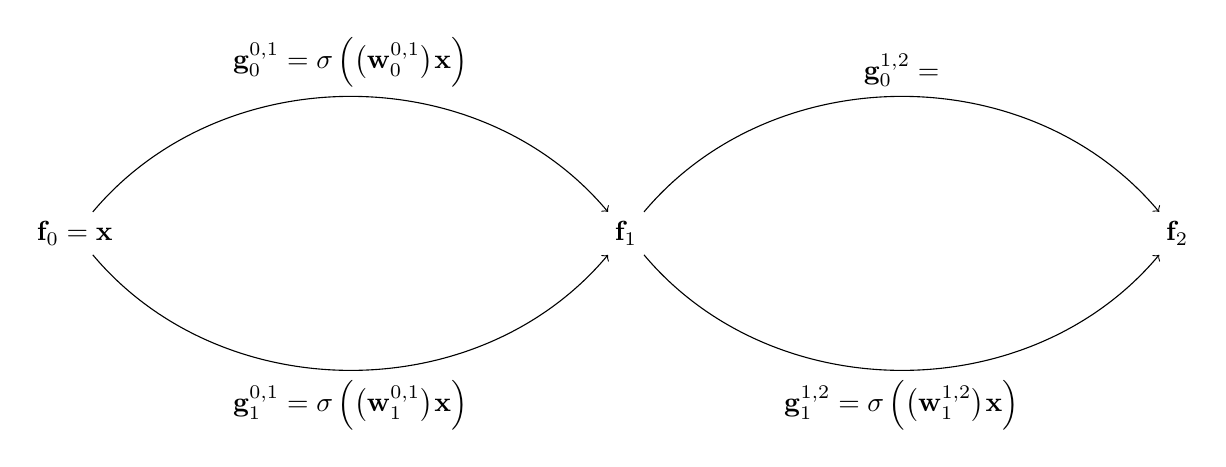
\begin{tikzpicture}[node distance=cm, auto]
  %\tikzstyle{every state}=[fill=red,draw=none,text=white]

  \node (f0)  at (1,3)                  {$\mathbf{f}_0 = \mathbf{x}$};
  \node (f1)  at (8,3)                  {$\mathbf{f}_1$};
  \node (f2)  at (15,3)                  {$\mathbf{f}_2$};
  %\node (f1)  at (6,4)                  {$\mathbf{f}_1$};
  %\node (f2)  at (6,2)                  {$\mathbf{f}_2$};

 %\node (f3)  at (10,3)                  {$\mathbf{f}_3$};
 %\node (f4)  at (15,3)                  {$\mathbf{f}_4$};

\path[->]  (f0) edge [bend left=50] node    {$\mathbf{g}^{0,1}_0 =  \boldsymbol{\sigma}\left({\bigl(\mathbf{w}^{0,1}_{0}\bigr)}^{\T}\mathbf{x}\right)$} (f1);
\path[->]  (f0) edge [bend right=50] node[below]    {$\mathbf{g}^{0,1}_1 =  \boldsymbol{\sigma}\left({\bigl(\mathbf{w}^{0,1}_{1}\bigr)}^{\T}\mathbf{x}\right)$} (f1);
\path[->]  (f1) edge [bend left=50] node    {$\mathbf{g}^{1,2}_0 =  \x$} (f2);
\path[->]  (f1) edge [bend right=50] node[below]    {$\mathbf{g}^{1,2}_1 =  \boldsymbol{\sigma}\left({\bigl(\mathbf{w}^{1,2}_{1}\bigr)}^{\T}\mathbf{x}\right)$} (f2);

%\path[->]  (f0) edge [bend right = 50]  node[below] {$\mathbf{g}^{0,2}_0 =  \boldsymbol{\sigma}\left({\bigl(\mathbf{w}^{0,2}_{0}\bigr)}^{\T}\mathbf{x}\right)$} (f2);
%\path[->]  (f1) edge [bend left = 50]  node {$\mathbf{g}^{1,3}_0 (\x) = \x$} (f3);
%\path[->]  (f2) edge [bend right = 50] node [below] {$\mathbf{g}^{2,3}_0 (\x) = \x$} (f3);
%\path[->]  (f3) edge [bend left = 50] node  {$\mathbf{g}^{3,4}_0 (\x) = \x$} (f4);
%\path[->]  (f3) edge [bend right = 50] node [below] {$\mathbf{g}^{3,4}_1 (\x) = \boldsymbol{\sigma}\left({\bigl(\mathbf{w}^{3,4}_{1}\bigr)}^{\T}\mathbf{x}\right)$} (f4); 


%\path[->]  (f2) edge node   {$\mathbf{g}^{2,3}_0 =  \textbf{softmax}$} (f3);


\end{tikzpicture}

\caption{Пример итерации алгоритма AdaNet~\cite{adanet}. Рассматривается две альтернативные модели: модель с углублением сети (соответствует выбору базовой функции $\mathbf{g}^{1,2}_1$  и модель с расширением сети (соответствует тождественной функции $\mathbf{g}^{1,2}_0$).} Базовая функция $\mathbf{g}^{0,1}_0$ была получена на предыдущей итерации алгоритма. В качестве функции агрегации для подмодели $\mathbf{f}_1$ выступает конкатенация: $\textbf{agg}_1 = \textbf{concat}$.
\label{fig:scheme_adanet}
\end{figure}

В работе~\cite{search_smbo} рассматривается задача порождения сверточных нейронных сетей. Предлагается проводить последовательный выбор структуры модели по восходящему числу параметров: начиная от сетей с одной подмоделью  и итеративно увеличивая количество подмоделей. В силу высокой вычислительной сложности данного подхода, вместо последовательного порождения моделей, предлагается провести оптимизацию рекуррентной нейронной сети, которая предсказывает качество модели по заданным подмоделям, и на основе данного предсказания выбрать наилучшую модель.
 
 
 
В работе~\cite{layer_probe} предлагается метод анализа структуры сети на основе линейных классификаторов, построенных на промежуточных слоях нейросети.
Схожий метод был предложен в~\cite{branches}, где классификаторы на промежуточных уровнях используются для уменьшения вычислений при выполнении вывода и предсказаний.
Промежуточные классификаторы работают как решающий список.

В работе~\cite{nn_inc} предлагается инкрементальный метод оптимизации нейросети. На первом этапе модель декомпозируется на несколько подмоделей, при которой модель последовательностью слоев $\mathbf{f}_1,\dots,\mathbf{f}_{|V|}$. Проводится последовательная оптимизация моделей вида:
\begin{enumerate}[1)]
\item $\mathbf{f} = \mathbf{f}_{|V|-1} (\mathbf{x});$
\item $\mathbf{f} = \mathbf{f}_{|V-2|} \circ \mathbf{f}_{|V|-1} (\mathbf{x});$
\item ...
\item $\mathbf{f} = \mathbf{f}_{0} \circ \dots \circ \mathbf{f}_{|V-1|} (\mathbf{x}).$
\end{enumerate}




\par{\textbf{Оптимизация структуры модели на основе обучения с подкреплением. }}
В~\cite{reinf} предлагается итеративная схема выбора архитектуры сверточной нейросети с использованием обучения с подкреплением. Распределение структур и параметров $\q$ задается рекуррентной нейронной сетью, которая определяет значение параметров модели и наличие ребер с ненулевыми операциями между вершинами графов модели. Параметры рекуррентной нейронной сети оптимизируются на основе значения функции $Q$, получаемого на каждой итерации алгоритма. Описанный метод также позволяет использовать в очередной подмодели результаты работы предыдущих подмоделей (англ. skip-connection). Пример параметрического семейства, описываемого в работе представлен на Рис.~\ref{fig:scheme_skip}.

\begin{figure}
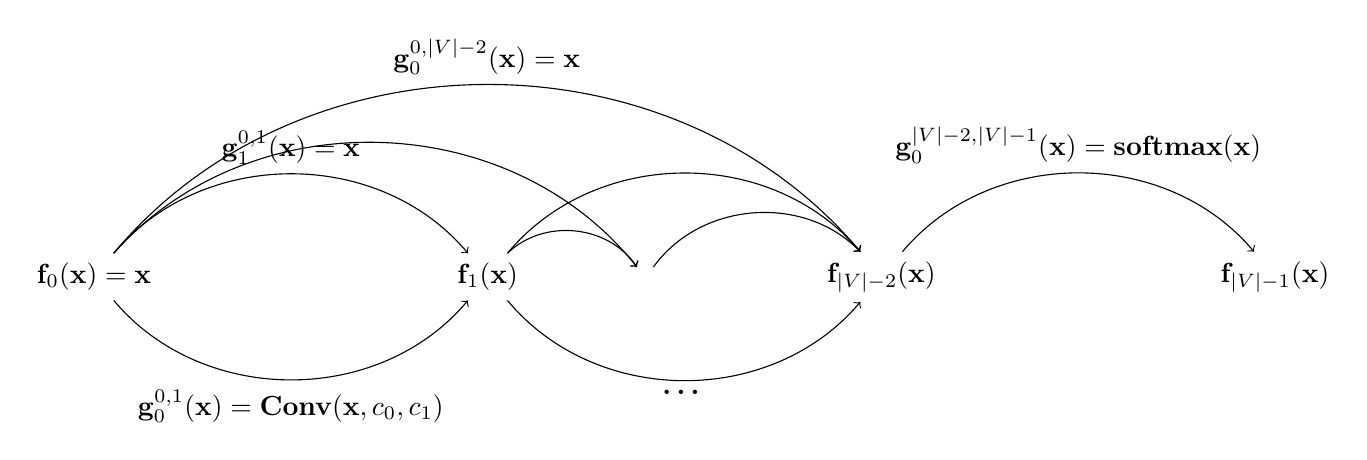
\begin{tikzpicture}[node distance=cm, auto]
  %\tikzstyle{every state}=[fill=red,draw=none,text=white]

  \node (f0)  at (1,6)                  {$\mathbf{f}_0(\mathbf{x}) = \mathbf{x}$};
 \node (f1)  at (6,6)                  {$\mathbf{f}_1(\mathbf{x})$};
 \node (fn1)  at (11,6)                  {$\mathbf{f}_{|V|-2}(\mathbf{x})$};
 \node (fn)  at (16,6)                  {$\mathbf{f}_{|V|-1}(\mathbf{x})$};
 \node (fdots)  at (8,6)                  {};
  \path[->]  (f0) edge [bend right=50] node[below] {$\mathbf{g}_0^{0, 1}(\mathbf{x}) = \textbf{Conv}(\mathbf{x}, c_0, c_1)$}(f1);
  \path[->]  (f1) edge [bend right=50] node[below] {\textbf{\dots}}(fn1);
  \path[->]  (f0) edge [bend left=50] node   {$\mathbf{g}_0^{0,|V|-2}(\mathbf{x})=\mathbf{x}$} (fn1);
  \path[->]  (f0) edge [bend left=50] node   {$\mathbf{g}_1^{0,1}(\mathbf{x})=\mathbf{x}$} (f1);
  \path[->]  (f0) edge [bend left=50]  (fdots);
  \path[->]  (f1) edge [bend left=50](fn1);
  \path[->]  (f1) edge [bend left=50] (fdots);
  \path[->]  (fdots) edge [bend left=50]  (fn1);

  \path[->]  (fn1) edge [bend left=50] node   {$\mathbf{g}^{|V|-2,|V|-1}_0(\mathbf{x})=\textbf{softmax}(\mathbf{x})$} (fn);

  %\path[->] (f0)  edge[bend right=50] node[below] {$\mathbf{g}^{1,2}(\mathbf{x}) = \boldsymbol{\sigma}(\mathbf{x}\mathbf{w}^{1,2})$}(f1);
  %\path[->] (f1)  edge node {$\mathbf{g}^{2,1}(\mathbf{x}) = \textbf{softmax}(\mathbf{x}\mathbf{w}^{2,1})$}(f2);       
  %\draw[->] (f1) to (f2);
 
\end{tikzpicture}


\caption{Пример параметрического семейства моделей глубокого обучения, описываемый в~\cite{reinf}. Каждая подмодель $\mathbf{f}_j$ является линейной комбинацией базовых функций: нелинейной функции и результата работы предыдущих подмоделей. }
\label{fig:scheme_skip}
\end{figure}



В работе~\cite{reinf_predict} предлагается алгоритм построения регрессионной модели для оценки финального качества модели и ранней остановки оптимизации моделей. Он позволяет существенно ускорить поиск моделей, представленный в~\cite{reinf}.
В~\cite{reinf_transfer} рассматривается задача переноса архитектуры нейросети, чья структуры была выбрана по выборке, меньшей мощности. Как и в~\cite{reinf} предлагается метод параметризации сверточной нейронной сети в виде графа. Предложенная параметризация позволяет задать более мощное параметрическое семейство моделей, чем в~\cite{reinf}. Модель представляется в виде последовательности суперпозиций подмоделей, называемых клетками (англ. normal cell и reduction cell). Каждая из этих клеток содержит следующее множество нелинейных операций $\mathbf{g}$, состоящее из тождественной операции $\mathbf{g}(\mathbf{x}) = \mathbf{x}$, а также множество сверток с фиксированным количеством каналов и размером фильтров и функций субдискретизации или пулинга.
Алгоритм выбора структуры модели рекуррентной сетью выглядит следующим образом на шаге $j$:
\begin{enumerate}[1)]
\item выбрать вершину $v'$ из вершин $v_{j-1}$, $v_{j-2}$ из данной клетки или вершину из предыдущих клеток;
\item выбрать вершину $v''$ из вершин $v_{j-1}$, $v_{j-2}$ из данной клетки или вершину из предыдущих клеток;
\item выбрать базовую функцию $\mathbf{g}'$ для применения к вершине $v'$;
\item выбрать базовую функцию $\mathbf{g}''$ для применения к вершине $v''$;
\item выбрать функцию агрегации результатов применения операций $\mathbf{g}',\mathbf{g}''$: сумму или конкатенацию.
\end{enumerate}


В отличие от предыдущих работ, в работе~\cite{reinf_deep2net} предлагается подход к инкрементальному обучению нейросети, основанном на модификации модели, полученной на предыдущем шаге. Рассматривается две операции над нейросетью: расширение и углубление сети.

В работах~\cite{net2net, morph, partition} рассматриваются методы деформации нейросетей. 
В работе~\cite{partition} предлагается метод оптимального разделения нейросети на несколько независимых сетей для уменьшения количества связей и, как следствие, уменьшения сложности оптимизации модели. В работе~\cite{net2net} предлагается метод сохранения результатов оптимизации нейросети при построении новой более глубокой или широкой нейросети. 
В работе~\cite{morph} рассматривается задача расширения сверточной нейросети, нейросеть рассматривается как граф.

В работе~\cite{darts} используется представление модели из~\cite{reinf_transfer}. Вместо обучения с подкреплением используются градиентная оптимизация структуры и параметров, выполненная в единой процедуре.

\section{Метаоптимизация моделей глубокого обучения}
Задача выбора структуры модели тесно связана с раздел машинного обучения под названием \textit{метаобучение} или \textit{метаоптимизация}. Под метаобучением понимаются алгоритмы машинного обучения~\cite{metalearn}, которые:
\begin{enumerate}[1)]
\item оценивают и сравнивают методы оптимизации моделей;
\item оценивают возможные декомпозиции процесса оптимизации моделей;
\item на основе полученных оценок предлагают оптимальные стратегии оптимизации моделей и отвергают неоптимальные. 
\end{enumerate}

В работе~\cite{self_rnn} предлагается подход к адаптивному изменению параметров сети. В качестве оператора оптимизации параметров рассматривается величина:
\[
    \TLoss = \boldsymbol{\theta} + \mathbf{f}_\text{optim}(\mathbf{f}_\text{mod}( \boldsymbol{\theta})),
\]
где $\mathbf{f}_\text{mod}$ --- функция, определяющая номер параметра из $\boldsymbol{\theta}$, подлежащего оптимизации, а $ \mathbf{f}_\text{optim}$ --- величина изменения параметра. 
В~\cite{self_rnn} также предлагается подмодель $\mathbf{f}_\text{ana}$, определяющая номер параметра, подлежащего дальнейшему анализу. Подход, описанный в данной работе, предполагает оптимизацию и анализ не только самой модели $\mathbf{f}$, но и дополнительных моделей $\mathbf{f}_\text{mod}, \mathbf{f}_\text{ana}, \mathbf{f}_\text{optim}$.

В работе~\cite{meta_sgd} рассматривается оптимизация метапараметров (шага градиентного спуска $\lambda_{\text{lr}}$ и начального распределения параметров $\boldsymbol{\theta}^0$). Рассматривается задача оптимизации параметров модели в случае, когда количество примеров невелико. Для этого проводится оптимизация параметров оператора оптимизации, который выглядит следующим образом:
\[
    \TLoss =  \boldsymbol{\theta}^0 - \boldsymbol{\lambda}\nabla  \TLoss[\teta^{0}],
\]
где векторы $\boldsymbol{\theta}^0$ и $\boldsymbol{\lambda}$ являются метапараметрами оператора $T$. Задача оптимизации параметров оператора $T$ рассматривается как задача многзадачного обучения (англ. multitask learning), когда оператор оптимизируется с учетом нескольких различных выборок и различных функций $L$, определенных отдельно для каждой выборки.


В работе~\cite{l2l} рассматривается задача восстановления параметров модели по параметрам  другой модели, чьи параметры были получены оптимизацией функции потерь на выборке меньшей мощности. Задачу можно рассматривать как задачу нахождения параметров некоторого оператора оптимизации $T$, действующего на параметры $\teta^0$, где $\boldsymbol{\theta}^0$ --- параметры модели, оптимизированной на небольшой выборке.  Предлагается функция оптимизации:
\[
   \TLoss  = \argmin \left(||\hat{\boldsymbol{\theta}} -  \boldsymbol{\theta}^0||_2^2 - \lambda \Loss[][\hat{\y}][\hat{\X}]\right),
\]
где $\boldsymbol{\theta}$ --- параметры модели, обученной по полной выборке $\mathfrak{D}$, $\hat{\mathfrak{D}}$ --- выборка меньшей мощности, ${\lambda}$ --- настраиваемый метапараметр.

В работе~\cite{l2l_by_gd_gd} рассматривается оптимизация метапараметров оператора оптимизации с помощью модели долгой краткосрочной памяти LSTM, которая выступает альтернативе аналитических алгоритмов, таких как Adam~\cite{adam} или AdaGrad~\cite{adagrad}. LSTM имеет небольшое число параметров, т.к. для каждого метапараметра используется свой экземпляр модели LSTM с одинаковыми параметрами для каждого экземпляра. Оптимизируемый функционал является суммой значений функции потерь $L$ на нескольких шагах оптимизации:
\[
   \Val = \sum_{t=1}^\eta \Loss[\teta^{t}],
\]
где $\eta$ --- число шагов оптимизации, $\boldsymbol{\theta}^t$ --- оптимизируемые параметры модели на шаге оптимизации $t$.


\section{Выбор структур моделей специального вида}
В данном разделе представлены работы по поиску оптимальных моделей со структурами специального вида.

В работе~\cite{mixed} рассматривается оптимизация моделей нейросетей с бинарной функцией активацией. Задача оптимизации сводится к задаче mixed integer программирования, которая решается методами выпуклого анализа.
В работе~\cite{energynet} предлагается метод построения сети глубокого обучения, структура которой выбирается с использованием обучения без учителя. Критерий оптимальности модели использует оценки энергетических функций и ограниченной машины Больцмана.

В работах~\cite{pathnet, supernet} рассматривается выбор архитектуры сети с использованием \textit{суперсетей}: связанных между собой подмоделей, образующих граф, каждый  путь из нулевой вершины в последнюю которого определяет модель глубокого обучения. Пример графа, описывающего суперсеть представлен на Рис.~\ref{fig:supernet}. В работе~\cite{supernet} рассматриваются стохастические суперсети, позволяющие выбрать структуру нейросети за ограниченное время оптимизации. 
Схожий подход был предложен в работе~\cite{pathnet}, где предлагается использовать эволюционные алгоритмы для запоминания оптимальных подмоделей и переноса этих моделей в другие задачи.


\begin{figure}
\centering
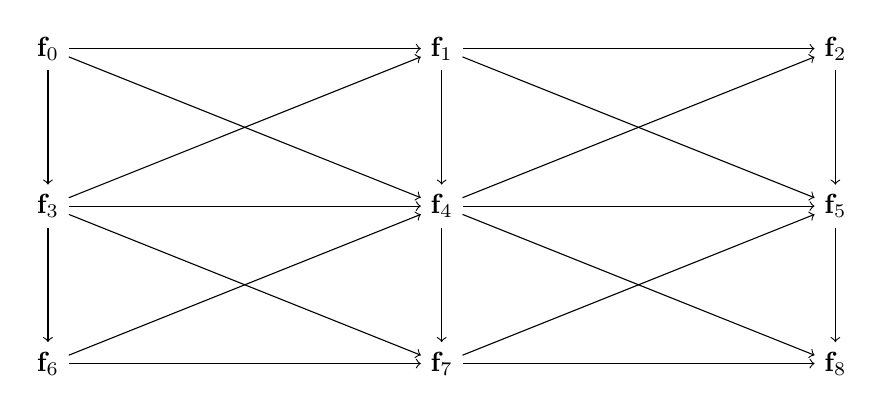
\begin{tikzpicture}[node distance=cm, auto]
  %\tikzstyle{every state}=[fill=red,draw=none,text=white]

  \node (f0)  at (1,5)                  {$\mathbf{f}_0$};
  \node (f1)  at (6,5)                  {$\mathbf{f}_1$};
  \node (f2)  at (11,5)                 {$\mathbf{f}_2$};

  \node (f3)  at (1,3)                  {$\mathbf{f}_3$};
  \node (f4)  at (6,3)                  {$\mathbf{f}_4$};
  \node (f5)  at (11,3)                 {$\mathbf{f}_5$};


  \node (f6)  at (1,1)                  {$\mathbf{f}_6$};
  \node (f7)  at (6,1)                  {$\mathbf{f}_7$};
  \node (f8)  at (11,1)                 {$\mathbf{f}_8$};

\path[->]  (f0) edge  (f1);
\path[->]  (f0) edge  (f3);
\path[->]  (f0) edge  (f4);
\path[->]  (f1) edge  (f2);
\path[->]  (f1) edge  (f4);
\path[->]  (f1) edge  (f5);
\path[->]  (f2) edge  (f5);
\path[->]  (f3) edge  (f1);
\path[->]  (f3) edge  (f4);
\path[->]  (f3) edge  (f6);
\path[->]  (f3) edge  (f7);
\path[->]  (f4) edge  (f2);
\path[->]  (f4) edge  (f5);
\path[->]  (f4) edge  (f8);
\path[->]  (f4) edge  (f7);
\path[->]  (f5) edge  (f8);
\path[->]  (f6) edge  (f7);
\path[->]  (f6) edge  (f4);
\path[->]  (f7) edge  (f5);
\path[->]  (f7) edge  (f8);
\end{tikzpicture}
\caption{Пример суперсети. Каждый путь из подмодели $\mathbf{f}_0$ в конечную модель $\mathbf{f}_8$ задает модель глубокого обучения.}
\label{fig:supernet}

\end{figure}

\textbf{Порождающие модели. }
Порождающими моделями называются модели, приближающие совместное распределение объектов и соответствующих им меток $p(\mathbf{X}, \mathbf{y})$. Частным случаем порождающих моделей являются модели, приближающие только распределение векторов объектов $\mathbf{X}$. Подобный случай будем считать частным случаем классификации при пустом множестве меток классов ($R=0$).

В качестве порождающих моделей в сетях глубокого обучения выступают ограниченные машины Больцмана~\cite{hinton_rbm} и автокодировщики~\cite{founds}. В работе~\cite{contractive} рассматриваются алгоритмы регуляризации автокодировщиков, позволяющих формально рассматривать данные модели как порождающие модели с использованием байесовского вывода. В работе~\cite{score} рассматриваются регуляризованные автокодировщики и свойства оценок их правдоподобия. В работе~\cite{vae} предлагается обобщение автокодировщика с использованием вариационного байесовского вывода~\cite{bishop}. В работе~\cite{train_generative} рассматриваются модификации вариационного автокодировщика и ступенчатых сетей~\cite{ladder} для случая построения многослойных порождающих моделей. 



В ряде работ~\cite{vae_graph,vae_stick,vae_mix,var_boost,layerwise_optimal} рассматривается подход к построению порождающих моделей глубокого обучения, при котором каждая подмодель $\mathbf{f}_i$ приближает распределение некоторой случайной величины $\mathbf{z}_i$, которая влияет на маргинальное распределение $p(\mathbf{X}, \mathbf{y}) = \int_{\mathbf{z}_0, \dots, \mathbf{z}_{|V|-1}} p(\mathbf{X}, \mathbf{y}|\mathbf{z}_0, \dots, \mathbf{z}_{|V|-1})p(\mathbf{z}_1, \dots, \mathbf{z}_{|V|})d\mathbf{z}_0\dots d\mathbf{z}_{|V|-1}.$ Подобный подход позволяет использовать вероятностную интерпретацию для каждой отдельной подмодели. 

В работе~\cite{vae_graph} рассматривается обобщение вариационного автокодировщика на случай более общих графических моделей. Предлагается проводить оптимизацию сложных графических моделей в единой процедуре. Для вероятностного вывода предлагается использовать нейронные сети.
Другая модификация вариационного автокодировщика представлена в работе~\cite{vae_stick}, авторы рассматривают использование процесса сломанной трости в вариационном автокодировщике, тем самым получая модель со стохастической размерностью скрытой переменной. В~\cite{vae_mix} рассматривается смесь автокодировщиков, где смесь моделируется процессом Дирихле.

В работе~\cite{var_boost} предлагается подход к оптимизации неизвестного распределения с помощью вариационного вывода. Предлагается решать задачу оптимизации итеративно, добавляя в модель новые компоненты вариационного распределения, проводится аналогия с бустингом.

В работе~\cite{layerwise_optimal} рассматривается задача построения порождающих моделей с дискретными значениями скрытой переменной ${z}$, предлагается критерий для послойного обучения порождающих моделей:
\[
    Q = \sum_{\mathbf{x} \in \X} \text{log} \sum_{i}p(\mathbf{x}|{z} = i)q({z}) \to \max,
\]
где $q$ --- аппроксимирующее распределение для случайной величины ${z}$, $i$ пробегает все значения переменной ${z}$.   

В работе~\cite{vae_ard} рассматривается метод ARD для снижения размерности скрытого пространства вариационных порождающих моделей. Скрытая переменная параметризуется как  произведение некоторой случайной величины $\mathbf{z}$  на вектор $\h$, отвечающий за релевантность каждой компоненты скрытой переменной. Схема порождения выборки $\mathbf{X}$ представлена на Рис.~\ref{fig:vae_ard}.

\begin{figure}[H]
\centering
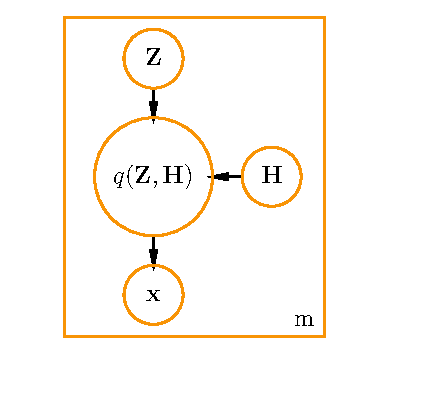
\includegraphics[width=0.25\textwidth]{./plots/notebooks/ae_plate.pdf}
\caption{Схема порождения вектора объектов $\mathbf{X}$, представленного в~\cite{vae_ard}.}
\label{fig:vae_ard}

\end{figure}

В данной работе предлагается метод последовательного порождения моделей глубокого обучения, основывающийся на применении вариационного вывода. Вариационный вывод позволяет получить оценки правдоподобия модели с небольшими вычислительными затратами, а также проследить потенциальное начало переобучения модели без использования контрольной выборки. Для регуляризации структуры модели предлагается ввести априорное распределение на структуре, позволяющее проводить оптимизацию модели и ее структуры в различных режимах. В качестве метода оптимизации гиперпараметров выступают градиентные методы, что позволяет эффективно производить оптимизацию большого числа гиперпараметров, сопоставимого с числом параметров модели. 

